% Uncomment for handout
\def\HANDOUT{}


\ifdefined\HANDOUT
\documentclass[handout]{beamer}
\usepackage{pgfpages}
\pgfpagesuselayout{4 on 1}[letterpaper,landscape,border shrink=5mm]
\else
\documentclass{beamer}
\fi

\mode<presentation>
{
  \usetheme{Warsaw}
  \definecolor{sered}{rgb}{0.78, 0.06, 0.18}
  \definecolor{richblack}{rgb}{0.0, 0.0, 0.0}
  \setbeamercolor{structure}{fg=sered,bg=richblack}
  %\setbeamercovered{transparent}
}


\usepackage[english]{babel}
\usepackage[latin1]{inputenc}
\usepackage{times}
\usepackage[T1]{fontenc}
\usepackage{tikz}
\usepackage{graphicx}
\usepackage[export]{adjustbox}
\usepackage{fancyvrb}
\usepackage{amsmath}
\usepackage{amssymb}
\usepackage{esvect}

\makeatletter
\newcommand{\imagesource}[1]{{\centering\hfill\break\hbox{\scriptsize Image Source:\thinspace{\tiny\itshape #1}}\par}}
\newcommand{\image}[3][\@nil]{%
        \def\tmp{#1}%
        \begin{center}
        \ifx\tmp\@nnil
            \includegraphics[max height = 0.55\textheight, max width = \textwidth]{images/#2}
        \else
            \includegraphics[max height = 0.50\textheight, max width = \textwidth]{images/#2}
            \linebreak
            #1
        \fi
        \linebreak
        {\tiny Image Source:\thinspace{\tiny #3}}
        \end{center}
}

\newenvironment{code}{%
 \VerbatimEnvironment
 \begin{adjustbox}{max width=\textwidth, max height=0.7\textheight}
 \begin{BVerbatim}
  }{
  \end{BVerbatim}
 \end{adjustbox}
}

\title{05 - Exploring Publications}


\author{Robert Lowe}

\institute[Southeast Missouri State University] % (optional, but mostly needed)
{
  Department of Computer Science\\
  Southeast Missouri State University
}

\date[]{}
\subject{}

\pgfdeclareimage[height=1.0cm]{university-logo}{images/semo-logo}
\logo{\pgfuseimage{university-logo}}



\AtBeginSection[]
{
  \begin{frame}<beamer>{Outline}
    \tableofcontents[currentsection]
  \end{frame}
}


\begin{document}

\begin{frame}
  \titlepage
\end{frame}

\begin{frame}{Outline}
  \tableofcontents
\end{frame}


% Structuring a talk is a difficult task and the following structure
% may not be suitable. Here are some rules that apply for this
% solution: 

% - Exactly two or three sections (other than the summary).
% - At *most* three subsections per section.
% - Talk about 30s to 2min per frame. So there should be between about
%   15 and 30 frames, all told.

% - A conference audience is likely to know very little of what you
%   are going to talk about. So *simplify*!
% - In a 20min talk, getting the main ideas across is hard
%   enough. Leave out details, even if it means being less precise than
%   you think necessary.
% - If you omit details that are vital to the proof/implementation,
%   just say so once. Everybody will be happy with that.

\section{Types of Publications}

\begin{frame}{Project Publication Order}
    \begin{enumerate}
        \item Poster
        \item Conference Paper
        \item Journal or Book Chapter
        \item Book
    \end{enumerate}
\end{frame}

\begin{frame}{Conferences}
    \begin{itemize}
        \item Classifications: Local, State, Regional, and International
        \item Can be either peer reviewed or general acceptance.
        \item Prestige often determined by size and acceptance rate.
        \item Two types of articles:
        \begin{itemize}
            \item \textbf{Poster} Presented during a poster session, and typically reports preliminary findings.
            \item \textbf{Conference Paper} Write and presentation presents a fully formed, but still new, idea.
        \end{itemize}
    \end{itemize}
\end{frame}

\begin{frame}{Journals}
    \begin{itemize}
        \item Journals contain long form articles.
        \item Journals are typically rated by impact factor:
        \[
        IF_y = \dfrac{Citations_y}{Publications_{y-1}+Publications_{y-2}}
        \]
        \item Types of journal articles:
        \begin{itemize}
            \item Original Research
            \item Short Reports or Letters
            \item Review Articles / Survey Articles
            \item Case Studies
            \item Methodologies and Methods
        \end{itemize}
    \end{itemize}
\end{frame}

\begin{frame}{Book Chapters}
    \begin{columns}
    
    \column{0.5\textwidth}
    \begin{itemize}
        \item Bound volumes of research.
        \item Similar to journals.
        \item One-Off, not periodical
    \end{itemize}
    
    \column{0.5\textwidth}
    \image{recent-trends}{Springer}
    
    \end{columns}
\end{frame}

\section{Citation Tracking}

\begin{frame}{Citation Tree}
    \begin{columns}
    \column{0.5\textwidth}
    \begin{itemize}
        \item Every article has sources.
        \item (Hopefully) Articles will be sources for others.
        \item Look forewords and backwards is important!
    \end{itemize}
    \column{0.5\textwidth}
    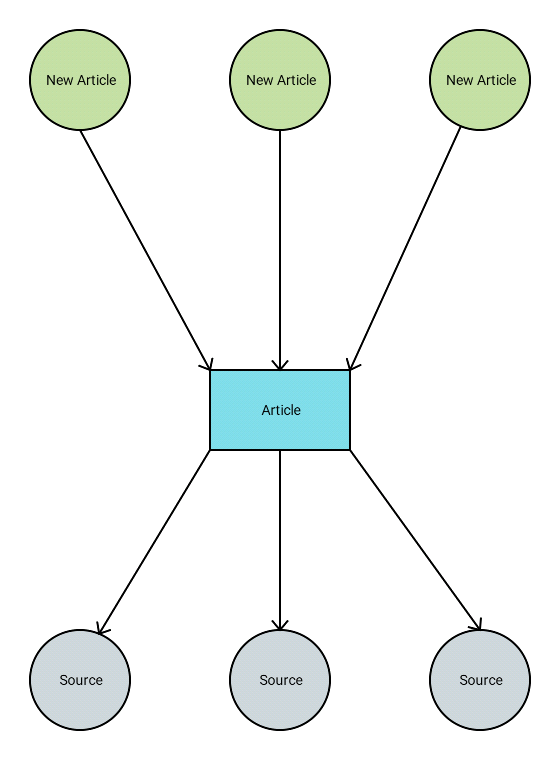
\includegraphics[width=\textwidth]{images/citations}
    \end{columns}
\end{frame}

\begin{frame}{Finding Citations}
    \begin{itemize}
        \item Most databases will list a document's citations.
        \item For going backwards, simply use the document's references.
        \item For going foreword, use tools such as Google Scholar's ``Cited By'' feature.
    \end{itemize}
\end{frame}
\end{document}
